%%%% Paramétrage du TD %%%%
\def\xxactivite{TD 02 \ifprof \\ Corrigé \else \fi }
\def\xxauteur{\textsl{Xavier Pessoles}}

\def\xxnumchapitre{Chapitre 3 \vspace{.2cm}}
\def\xxchapitre{\hspace{.12cm} Précision des systèmes}

\def\xxcompetences{%
\textsl{%
\textbf{Savoirs et compétences :}\\
\vspace{-.4cm}
%\begin{itemize}[label=\ding{112},font=\color{bleuxp}] 
%\item \textit{Mod3.C2 : } pôles dominants et réduction de l’ordre du modèle : principe, justification
%\item \textit{Res2.C4 : } stabilité des SLCI : définition entrée bornée -- sortie bornée (EB -- SB)	
%\item \textit{Res2.C5 : } stabilité des SLCI : équation caractéristique	
%\item \textit{Res2.C6 : } stabilité des SLCI : position des pôles dans le plan complexe
%\item \textit{Res2.C7 : } stabilité des SLCI : marges de stabilité (de gain et de phase)
%\end{itemize}
}}
\def\xxtitreexo{Segway}
\def\xxsourceexo{\hspace{.2cm} \footnotesize{Editions Vuibert.}}

\def\xxfigures{
\begin{center}
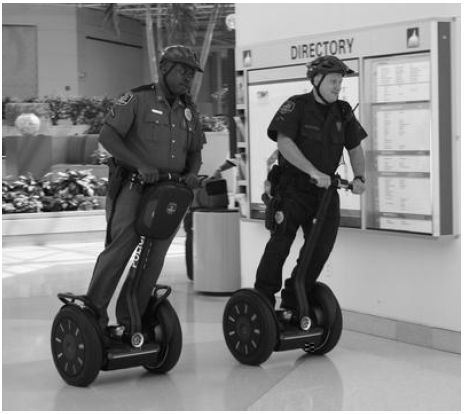
\includegraphics[width=.5\textwidth]{segway.png}
\end{center}
%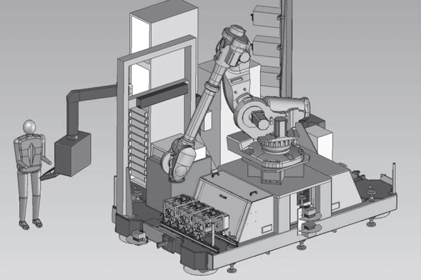
\includegraphics[width=.4\linewidth]{image1}
}%figues de la page de garde

\input{\repRel/Style/pagegarde_TD}
\setlength{\columnseprule}{.1pt}

\pagestyle{fancy}
\thispagestyle{plain}


\vspace{4.5cm}

\def\columnseprulecolor{\color{bleuxp}}
\setlength{\columnseprule}{0.4pt} 

%%%%%%%%%%%%%%

\setcounter{numques}{0}

\begin{multicols}{2}

\section*{Analyser le besoin et la structure du système\\}


Le Segway\textregistered{} est un moyen de transport motorisé qui permet de se déplacer en ville. En terme de prestations,
il est moins rapide qu'une voiture ou qu'un scooter, plus maniable, plus écologique, moins encombrant
et nettement plus moderne.

La conduite du Segway\textregistered{} se fait par inclinaison du corps vers l'avant ou vers l'arrière, afin d'accélérer
ou freiner le mouvement. Les virages à droite et à gauche sont, quant à eux, commandés par l'inclinaison
du guidon.

La spécificité de ce véhicule est d'avoir deux roues qui ont le même axe de rotation, avec son centre
de gravité situé au-dessus de l'axe commun des roues, si bien qu'on se demande comment rester à
l'équilibre une fois monté sur la plate-forme. Tout comme le cerveau permet à l'homme de tenir debout
sans tomber grâce à l'oreille interne, le système comporte un dispositif d'asservissement d'inclinaison,
maintenant la plate-forme du véhicule à l'horizontale ou encore la barre d'appui, supposée orthogonale
à cette plate-forme, à la verticale.

\normalsize

\subsection*{ Cahier des charges} Les exigences attendues pour le Segway\textregistered{} sont listées sur le diagramme de la figure suivante.%ref{ex_Segway_exigences}.

\begin{center}%\begin{figure}[!ht]
%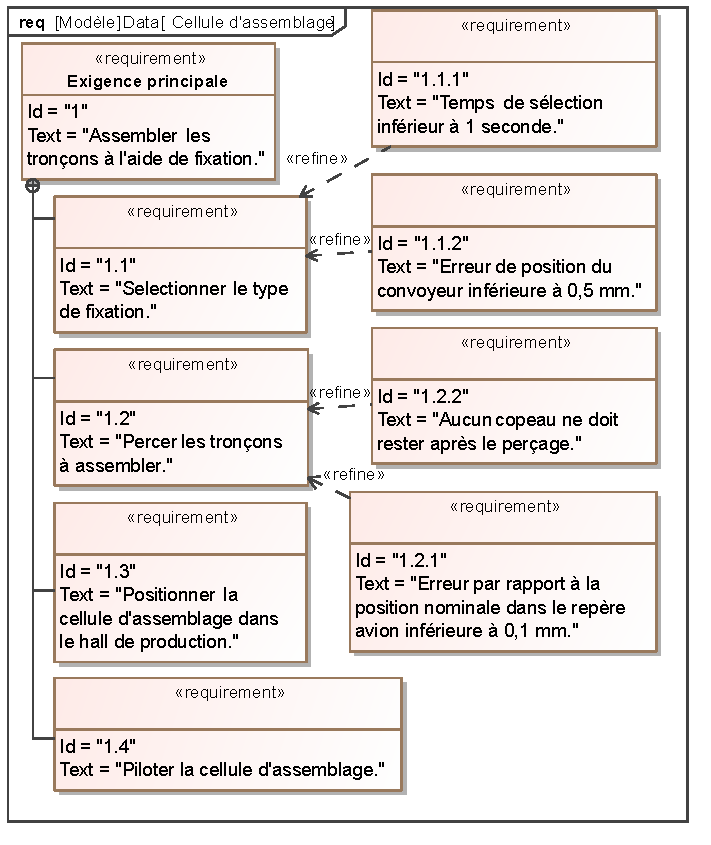
\includegraphics[width=1.\textwidth]{Exigences}

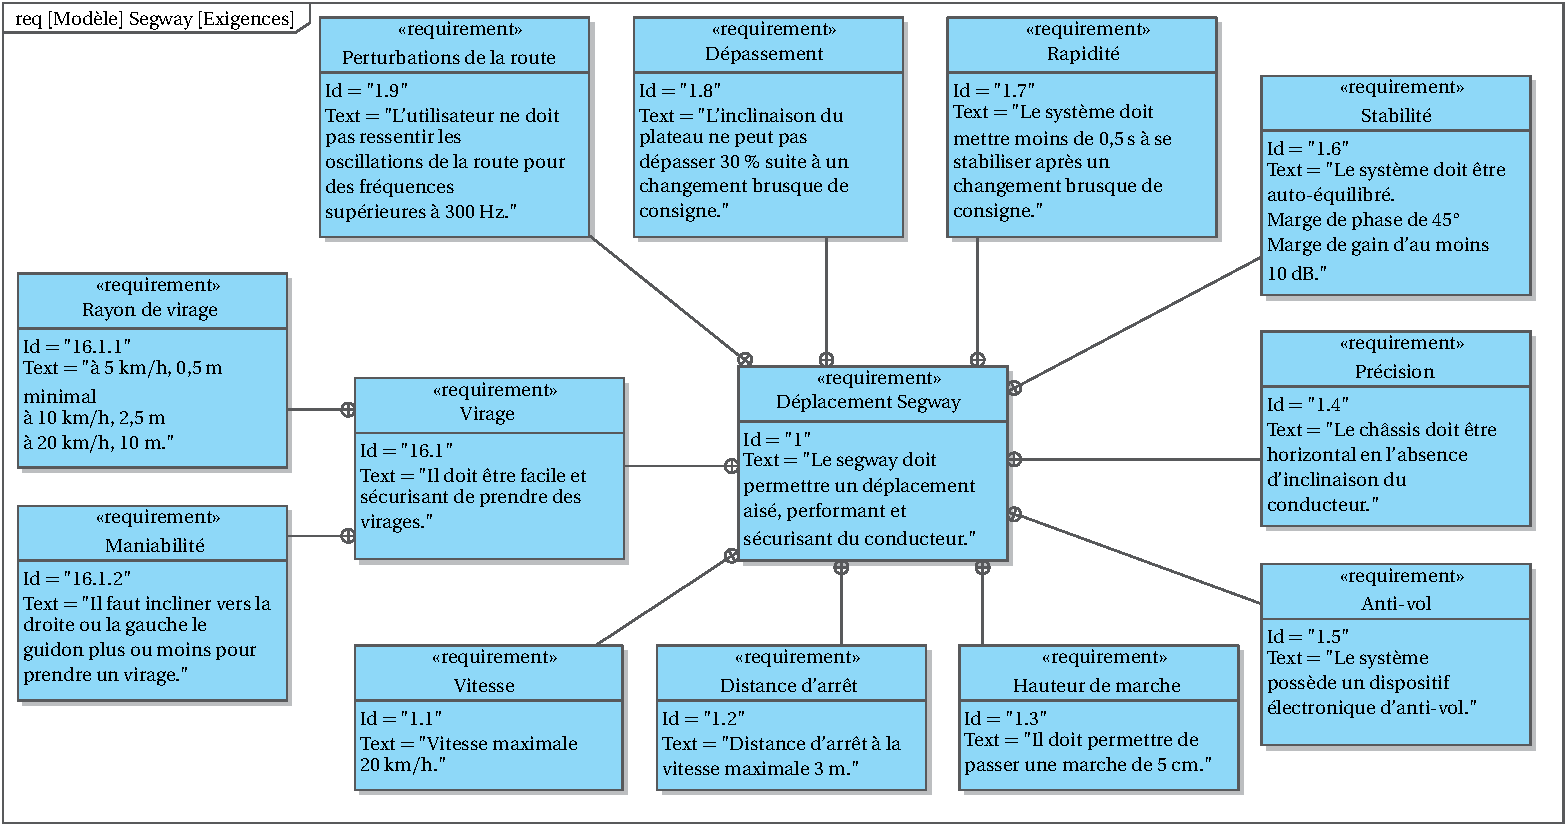
\includegraphics[width=\linewidth]{Diagramme_Exigences}
\textit{Diagramme des exigences du Segway\textregistered.}
\label{ex_Segway_exigences}
\end{center}%\end{figure}[!ht]



Le diagramme BDD de la figure ci-après montre les constituants du Segway\textregistered.


\begin{obj}
La difficulté essentielle de ce système est d'être capable de maintenir le chariot stable tout en ayant de bonnes performances. L'objectif du travail proposé est de vérifier qu'un asservissement correctement réglé permet de respecter les critères de stabilité, précision et rapidité définis dans le diagramme des exigences.
\end{obj}


\begin{center}%\begin{figure}[!ht]
%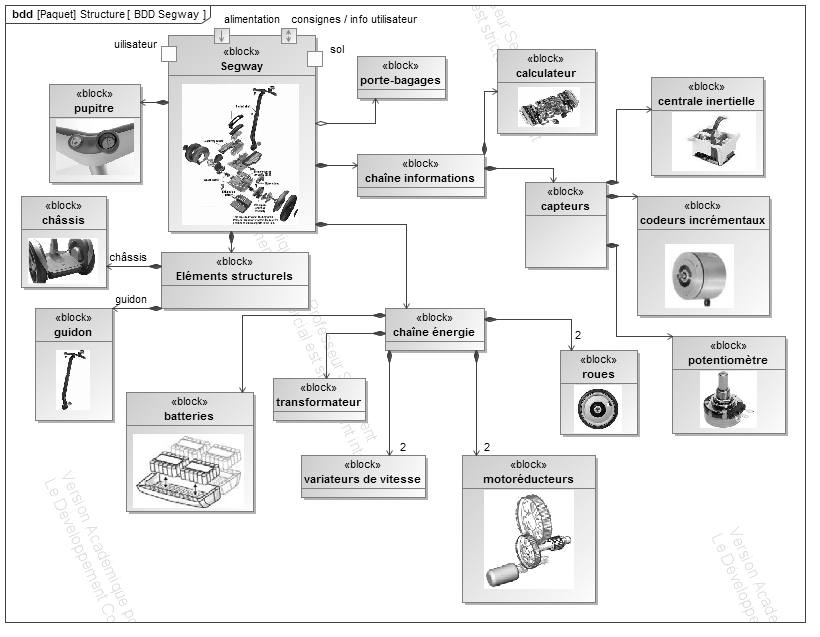
\includegraphics[width=1.\textwidth]{BDD}
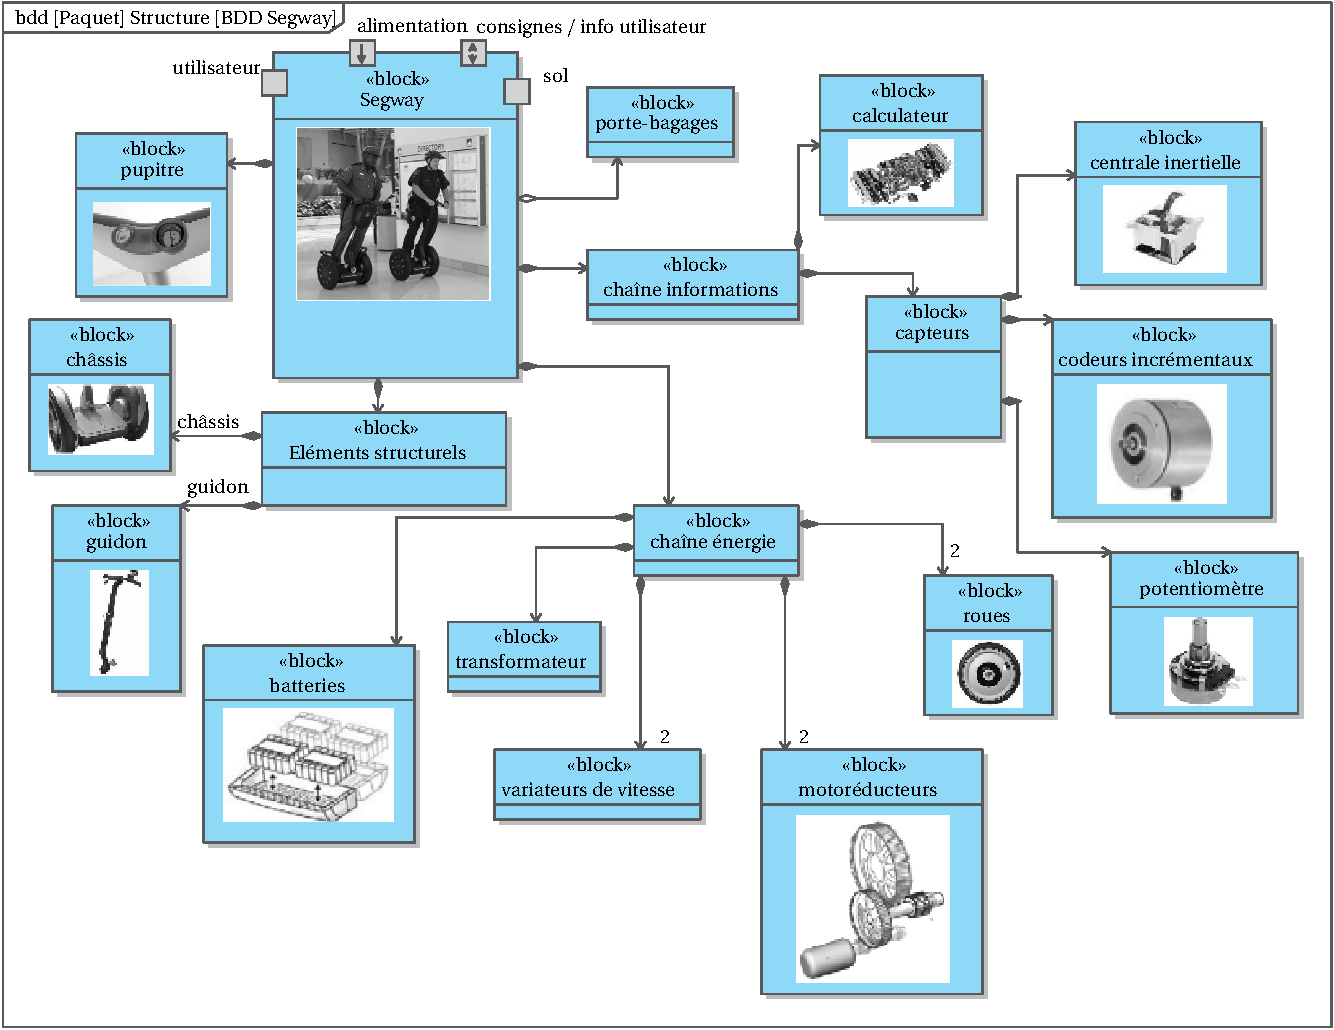
\includegraphics[width=\linewidth]{Diagramme_BDD}
\textit{Diagramme de définition des blocs du Segway\textregistered.}
\label{ex_Segway_BDD}
\end{center}%\end{figure}[!ht]



\subsection*{Modéliser le système}

On donne le schéma-blocs proche de l'architecture retenue pour le système.% est donné sur la figure \ref{segway_sb1}.

\begin{center}%\begin{figure}[!ht]
%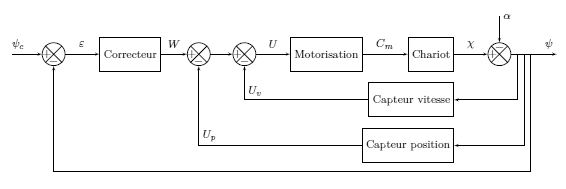
\includegraphics[width=1.\textwidth]{Modelisation_segway}
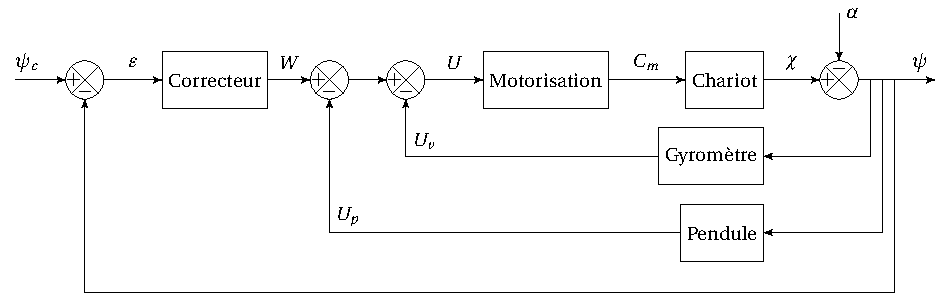
\includegraphics[width=\linewidth]{segway_sb_causal}
\textit{Schéma-blocs fonctionnel du Segway\textregistered.}
\label{segway_sb1}
\end{center}%\end{figure}[!ht]

Les équations (simplifiées) caractérisant les différents sous-systèmes sont les suivantes :
\begin{itemize}
\item ensemble amplificateur et motoréducteur :  $C_m(t)=K_m u(t)$ avec $K_m=\SI{2}{Nm V^{-1}}$;
\item ensemble chariot + conducteur :  $a\dfrac{\dd^2 \chi(t)}{\dd t^2}=bC_m(t)+c \chi(t)$ (avec $a$, $b$ et $c$ constantes positives); 
\item gyromètre :  $u_v(t)=k_v \dfrac{\dd\chi(t)}{\dd t}$;
\item pendule :  $u_p(t)=k_p \chi(t)$.
\end{itemize}



\question{Déterminer, à l'aide des équations de chaque constituant, les fonctions de transfert de chaque bloc du schéma-blocs.}% de la figure \ref{ex_segway_SB}.}

\begin{center}%\begin{figure}[!ht]
%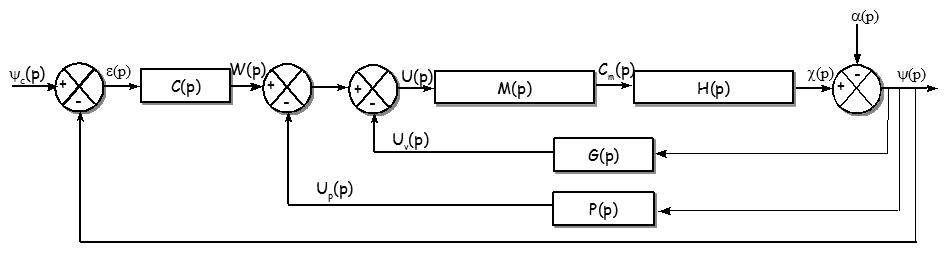
\includegraphics[width=.7\textwidth]{schema_bloc.png}
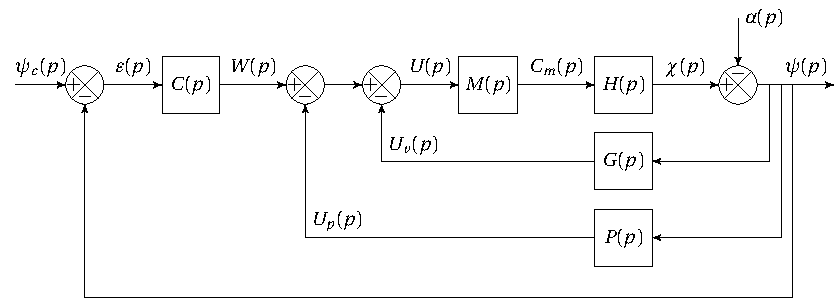
\includegraphics[width=\linewidth]{segway_sb_causal2}
\textit{Schéma-blocs du Segway\textregistered.} \label{ex_segway_SB}
\end{center}%\end{figure}[!ht]

\question{Mettre la fonction de transfert du chariot $H(p)$ sous la forme canonique $H(p)=\frac{K_1}{\frac{p^2}{\omega_1^2}-1}$. On prendra pour la suite $K_1=\SI{0.12}{rad. N.m^{-1}}$ et $\omega_1=\SI{4.1}{rad. s^{-1}}$.}

\question{Justifier que le chariot seul est un système instable.}

\section*{Paramétrer la FTBO}

On prend $F(p)=\frac{\num{0.12}}{1+\num{0.23} p + \num{0.026} p^2}$ et $K_C=5,47$ (permettant de garantir la marge de  \SI{-135}{\degree}) .

%%
%%\question{Déterminer la Fonction de Transfert en Boucle Ouverte du système $\textrm{FTBO}(p)=\frac{\Psi(p)}{\varepsilon(p)} = C(p)F(p)$ où l'on précisera $F(p)$ en fonction des paramètres $K_m$, $K_1$, $\omega_1$, $k_v$ et $k_p$.}
%%\question{Pour pouvoir appliquer le critère du revers, il faut que la FTBO ne possède que des pôles à partie réelle négative. Quelle condition doit-on avoir sur les coefficients de $F(p)$ ? Y a-t-il d'autres conditions à respecter pour que le système ainsi asservi soit stable de façon absolue (sans vérifier si les valeurs des marges sont suffisantes) si on prend $C(p)=1$ ?}
%%Les paramètres $k_v$ et $k_p$ sont choisis de manière à assurer, non seulement la stabilité du système, mais aussi sa rapidité.
%%\question{\`A partir de l'expression de $F(p)$, déterminer les paramètres $k_v$ et $k_p$ permettant d'assurer une rapidité optimale en boucle ouverte en prenant une pulsation $\omega_0=\num{1.5} \omega_1$. }
%%Dans la suite, la fonction $F(p)$ utilisée sera la suivante $F(p)=\frac{\num{0.12}}{1+\num{0.23} p + \num{0.026} p^2}$.

%%On choisit un correcteur proportionnel $C(p)=K_c$.

%%\question{Déterminer analytiquement la pulsation et le gain correspondant à une phase de \SI{-135}{\degree}. Que dire de la marge de gain en fonction de la valeur de $K_c$.}

%%\question{En déduire la valeur à prendre pour $K_c$ de manière à respecter le cahier des charges vis-à-vis de la stabilité (marge de phase).}


\subsection*{Caractériser les performances du système complet}

Afin d'assurer l'asservissement, la régulation d'inclinaison du Segway\textregistered{} délivre une consigne $\psi_c$ nulle.  Cette régulation est satisfaisante si, quelle que soit l'inclinaison $\alpha$ du conducteur, la sortie $\psi$ converge vers $\psi_c$, de valeur nulle ici.  Le paramètre $\alpha$ peut donc être considéré comme une perturbation.



\question{Déterminer la fonction de transfert $H_r(p)=\frac{\Psi(p)}{\alpha(p)}$.}

\begin{center}%\begin{figure}[!ht]
%\includegraphics[width=.7\textwidth]{bode.png}
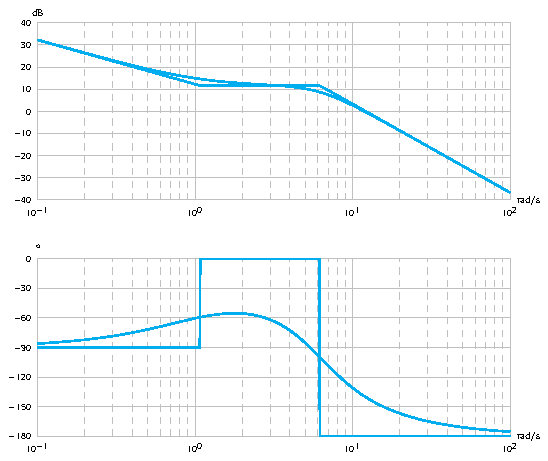
\includegraphics[width=\linewidth]{segway_bode}
%\textcolor{red}{DV : tracer les diag de bode de C(p).F(p) avec F défini plus haut et C défini au dessus.}
\textit{Diagrammes de Bode de la FTBO corrigée.} \label{ex_Segway_bode}
\end{center}%\end{figure}[!ht]

\question{Calculer l'inclinaison $\psi$ du châssis en régime permanent, lorsque la perturbation $\alpha$ est un échelon d'amplitude $\alpha_0=\SI{20}{\degree}$ pour le correcteur $K_c$ défini précédemment. Le cahier des charges est-il satisfait ?}

\question{On utilise alors un correcteur proportionnel intégral de la forme $C(p)=K_i \frac{1+T_i p}{T_i p}$ (le réglage d'un tel correcteur sera vu dans un chapitre ultérieur) avec $K_i=\num{31.7}$ et $T_i=\SI{0.93}{s}$. Justifier que ce correcteur améliore la robustesse ainsi que la précision.}

Les diagrammes de Bode de la nouvelle FTBO sont donnés sur la figure suivante.% \ref{ex_Segway_bode}.


\question{Vérifier que la stabilité est toujours respectée avec ce réglage de correcteur.}



\subsection*{Retour sur le cahier des charges}
\begin{center}
%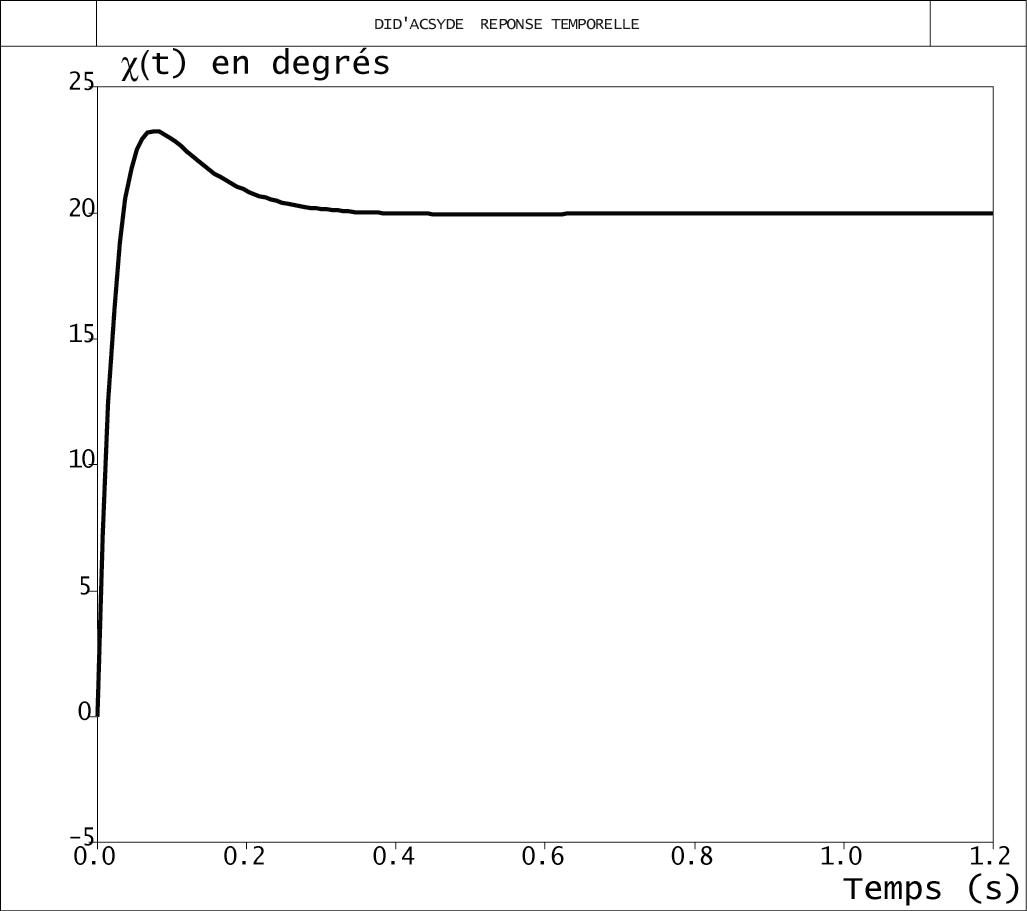
\includegraphics[width=.9\textwidth]{reponse_temporelle.png}
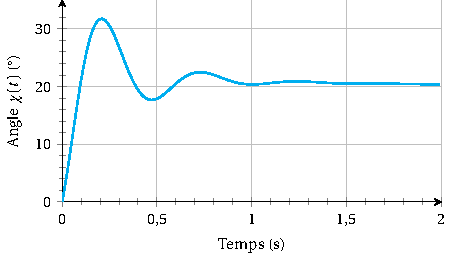
\includegraphics[width=.9\linewidth]{systeme_corrige_reponse}
\textit{Réponse temporelle $\chi(t)$ pour une entrée en échelon $\alpha=\SI{20}{\degree}$.}
\label{ex_segway_reponse_temporelle}
\end{center}




La courbe précédente % Figure \ref{ex_segway_reponse_temporelle} 
correspond à l'évolution de l'angle $\chi(t)$ au cours du temps pour une consigne en échelon $\alpha=\SI{20}{\degree}$ pour le correcteur retenu. Vérifier que les critères de stabilité, rapidité, précision et dépassement du cahier des charges sont respectés.









\ifcolle
\else
\subsection*{Éléments de correction}
\begin{enumerate}
\item $H_{\Omega}(p)=\dfrac{\dfrac{1}{K_{\Omega}}\left( 1 + T_{1}p \right)}{\dfrac{T_{1} K_{rI}J}{K_{\Omega}k_{1}K}p^2+\left(\dfrac{f K_{rI}}{K_{\Omega}k_{1}K}+1\right)T_{1}p + 1 }$.
\item  $b=\dfrac{1}{K_{\Omega}} = 20 \pi = \SI{62,8}{rad.s{-1}V^{-1}}$ et $\tau=\dfrac{K_{ri}J}{k_1KK_{\Omega}}=\SI{2,17e-3}{s}$.
\item $\dfrac{T_{1}K_{ri}p}{ k_{1}\left( T_{1}p + 1 \right)K}\cdot \dfrac{b}{p\left(1+\tau p \right)+b}$ et $\lim\limits_{t\to\infty} \theta(t) = 1$.
\item  ${a}=\dfrac{1}{4bc\tau\xi^2}=0,092$.
\item $\mu(p)=\dfrac{p\left( 1+\tau p\right)}{p\left( 1+\tau p\right)+abc}\theta_c(p)$, $\mu_p = 0$, $\mu_v = \dfrac{1}{abc}$ et  $\mu_a = \infty$.
\item $\mu_p=0$ et $\mu_v= \dfrac{1 -bd}{ab}$.
\item ...
\item ...
\item ...
\item ...
\end{enumerate}
\fi

\end{multicols}


%\begin{center}
%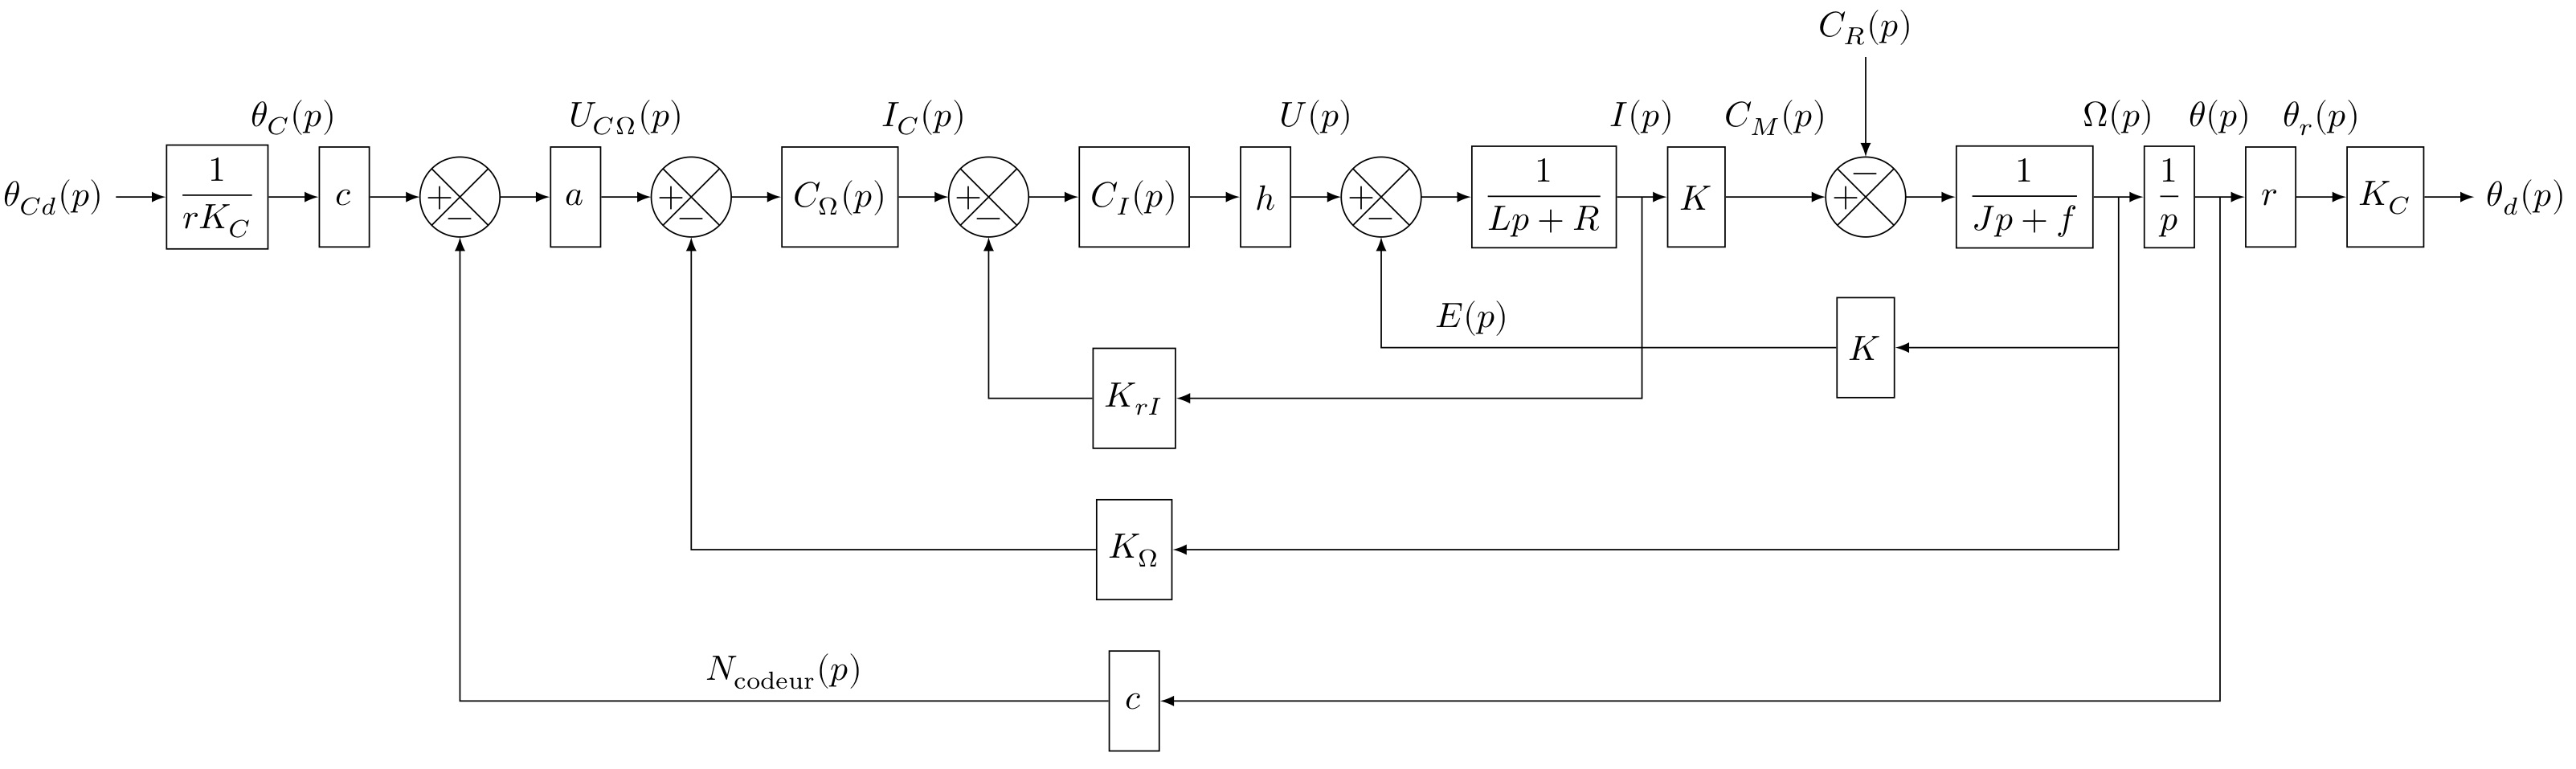
\includegraphics[width=\linewidth]{schema_bloc.jpg}
%
%\textit{Schéma-blocs de l'asservissement du dosseret \label{fig6}}
%\end{center}

%\end{document}
%
%\question{}
%\ifprof
%\begin{corrige}
%\end{corrige}
%\else
%\fi
%
%\begin{center}
%\includegraphics[width=\linewidth]{}
%%\textit{}
%\end{center}
%\begin{center}
%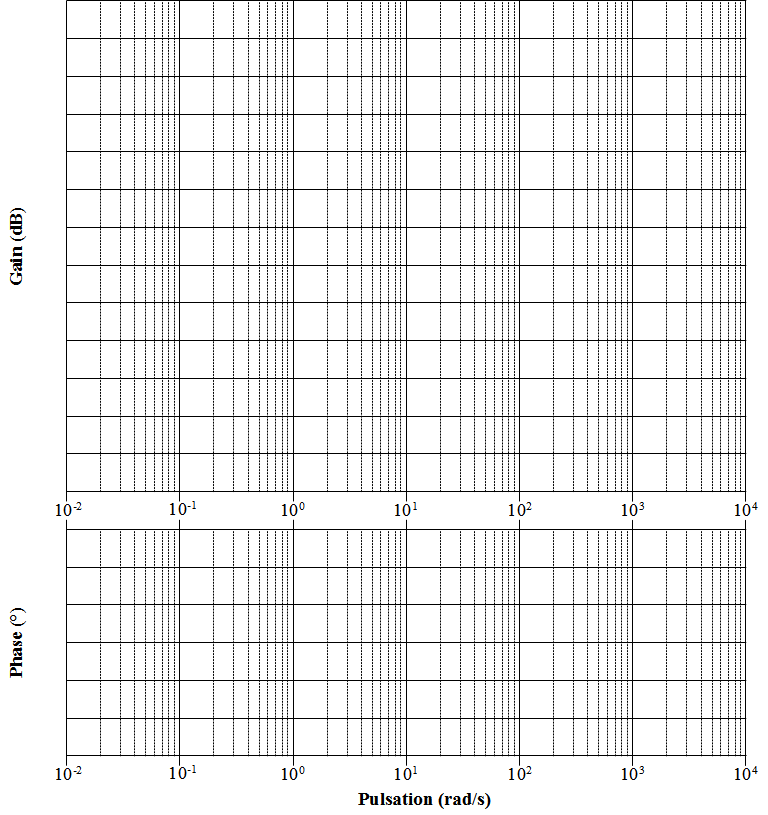
\includegraphics[width=\linewidth]{img_04}
%%\textit{}
%\end{center}
%
